\documentclass{report}
\usepackage{amsmath}
\usepackage{graphicx}
\usepackage{color}
\begin{document}

\chapter{General Introduction}
Sooner or later, every scientist or engineer runs into the problem
of having to find the ``best'' solution some set of decisions can
give. Usually, the variables governing such problems are related
to one another in a rather complicated way, and finding the
``best'' combination of them can seem intractable. Normally, the
relations between these decision variables can be translated into
so-called \emph{objective functions}, and the value of each of
these functions can be interpreted as a measure of the quality
that particular combination of the decision variables give to a
particular aspect of the solution.
\\�\\
As such, $N$-dimensional optimization problems with $m$ individual
objective functions can be stated generally as

\[
\textrm{find } "\min" F(x) = \begin{bmatrix}
         f_1(x)\\ f_2(x)\\ \vdots\\ f_m(x)
         \end{bmatrix}
\]

subject to

\begin{eqnarray*}
G(x) &<& 0  \\
H(x) &=& 0   \\
lb \leq &x& \leq ub,
\end{eqnarray*}

where

\[
x = \left[x_1,\,x_2,\,\ldots,\,x_N\right],
\]

and $f_1(x)$ through $f_m(x)$ indicate the individual objective
functions. In almost all practical cases, finding good solutions
is not a problem, but finding the \emph{best} solution is much
more difficult. Moreover, for most problems encountered in
practice, the objective functions $f_1(x)$ through $f_m(x)$ are
highly nonlinear, non-smooth, non-differentiable, or have no way
of determining initial estimates close to the global optimum, or a
combination of all of these factors.
\\�\\
The only practical solution to tackle such problems is to use a
so-called \emph{meta-heuristic optimizer}, which uses a
``population'' of trial solutions, and applies certain
probabilistic rules to generate a new population which converges
to the global minimum of the objective function with high
probability. Over the years, many such algorithms have been
developed, of which the Genetic Algorithm (GA), Differential
Evolution (DE), Particle Swarm Optimization (PSO) and Adaptive
Simulated Annealing (ASA) received more attention.
\\�\\
Although meta-heuristic optimization algorithms usually require
quite many function evaluations, their popularity grew enormously
due to their ability to find global optima even in extremely
difficult problems and with relatively low population sizes.
Moreover, their elegance and simplicity appealed to many people --
a thorough understanding of other optimization algorithms that
existed at the time (which were much harder to implement, and did
not always find the \emph{global} optimum), was no longer
required, and problems could be optimized much faster (and usually
much better) than was previously possible.

\chapter{Single-objective Optimization}
Originally, the aforementioned meta-heuristic algorithms were
intended for problems with $m = 1$ (referred to as
single-objective optimization); their aim is to find the global
minimum of a \emph{single} objective function. Many problems can
indeed be stated as a single objective problem:

\[
\textrm{find } \min F(x)
\]

subject to

\begin{eqnarray*}
G(x) &<& 0\\
H(x) &=& 0 \\
lb < &x& < ub
\end{eqnarray*}

and $x = \left[x_1,\, x_2,\, \ldots,\,x_N\right]$ as before.
Meta-heuristic algorithms first create a population of randomly
generated solutions,

\[
pop = \begin{bmatrix}
         x_{11} & x_{21} & x_{31} & \ldots & x_{N1}\\
         x_{12} & x_{22} & x_{32} & \ldots & x_{N2}\\
         &&\vdots&&\\
         x_{1P} & x_{2P} & x_{3P} & \ldots & x_{NP}
         \end{bmatrix}
\]

where each $x_{ij}$ is taken within the preset boundaries $[lb]$
and $[ub]$ (the constraints $G(x)<0$ and $H(x) =0$ are then
usually added to $F(x)$ in the form of \emph{penalty functions}).
The objective function $F(x)$ is evaluated for each member in this
population, and a new population is created based on the function
values of the initial population, and a certain degree of
randomness. The four aforementioned algorithms do this as follows:

\section{GA (based on natural evolution)}

\begin{enumerate}

\item Select two individuals that function as parents, say
individuals 2 and 8.

\item split the parents in two, at some random location $CR$:
\begin{eqnarray*}
         parent1 &=& [x_{18},\, x_{28},\, \ldots, x_{CR8},\,\ldots,\,x_{N8}]\\
         parent2 &=& [x_{12},\, x_{22},\, \ldots, x_{CR2},\,\ldots,\,x_{N2}]\\
\end{eqnarray*}

\item Let the parents \emph{crossover} at the point $R$ (with a
certain probability $p_{cross}$) to create two children:
\begin{eqnarray*}
         child1 &=& [x_{18},\, x_{28},\, \ldots, x_{CR2},\,\ldots,\,x_{N2}]\\
         child2 &=& [x_{12},\, x_{22},\, \ldots, x_{CR8},\,\ldots,\,x_{N8}]\\
\end{eqnarray*}

\item Do this until $P$ children have been created.

\item \emph{Mutate} the children, with a certain (small)
probability $p_{mutate}$. This selects a few random indices ($M$)
in ALL children, and replaces the associated values with random
other values (randomly selected from the interval $[lb,\, ub]$):
\begin{eqnarray*}
         child1 &=& [x_{18},\, x_{28},\, \ldots, x_{CR2},\,\ldots,\,xM2,\,\ldots x_{N2}]\\
         child2 &=& [x_{12},\, x_{22},\, \ldots, x_{CR8},\,\ldots,\,x_{N8}]\\
\end{eqnarray*}

\item Evaluate the objective function for all the children. If a
child is found to have a ``better'' function value than either of
its parents, it will become part of the new population. Otherwise,
the better of the two parents is inserted into the new population.

\end{enumerate}

Steps 1-6 are repeated until ``convergence''.
\\�\\
The original GA used a \emph{binary} representation of the
population, i.e., each individual is represented by \emph{bits} in
stead of real numbers. Crossover and mutation are also carried out
bit wise, that is

\begin{eqnarray*}
     parent1 &=& [10110011010010\ldots00110110001001]\\
     parent2 &=& [11001110110011\ldots00110011111001]\\
\textrm{crossover }&\rightarrow& \\
     child1 &=& [10110011010010\ldots\textcolor{blue}{00110011111001}]\\
     child2 &=& [11001110110011\ldots\textcolor{blue}{00110110001001}]\\
\textrm{mutation }&\rightarrow&   \\
     child1 &=& [10110011010010\ldots001\textcolor{red}{0}0011111001]\\
     child2 &=& [110\textcolor{red}{1}1110110011\ldots0011011000100\textcolor{red}{0}]
\end{eqnarray*}

Whether to use binary representation or real numbers usually
depends on the problem. For lower dimensionality ($N$ is small) it
is usually more efficient to use binary representation, and when
the population size is enormous it is more efficient to use real
numbers to avoid the costly conversion to binary and back, etc.
But these ``rules-of-thumb'' usually need to be tested for each
new problem.

\section{DE (based on globalized pseudo-derivatives)}

\begin{enumerate}

\item Randomly select three individuals from the population, say
3, 7 and 15. These individuals will function as the \emph{base
vector} and \emph{differentiation vectors}, respectively.

\item The $i^\textrm{th}$ individual is created according to the
rule

\[
\begin{array}{ll}
\texttt{if rnd < }Cr&\\
 & ind = pop(3,\,:) + F(pop(7, :) - pop(15,\,:))\\
\texttt{else}&\\
& ind = pop(i,\,:) \\
\texttt{end}&
\end{array}
\]

where \texttt{rnd} is a random number, $Cr$ is the \emph{crossover
probability}, and $F$ the \emph{constant of differentiation},
usually a random number in $[-1,\,1]$.

\item Do this until $P$ new individuals have been created.

\item Evaluate the objective function for all these new
individuals. If a new individuals is found to have a ``better''
function value than its spawning solution, it will become part of
the new population. Otherwise, the original vector is inserted.

\end{enumerate}

Taking the \emph{difference} between the two differentiation
vectors is very much like taking the derivative. But as the two
differentiation vectors are usually quite far apart (certainly not
infinitesimally far), this ``derivative'' is more a global measure
of how much the objective function changes \emph{on average} over
that interval. The derivative is computed at each iteration
between two new, \emph{randomly} selected vectors, so on average,
the solutions will tend to go to where the average slope is zero,
and the function globally minimal. Sometimes this operation is
called the \emph{global pseudo-derivative}, and it is the key to
the power of the DE algorithm.
\\�\\
Numerous variations on this basic algorithm exist. However, they
normally improve DE's performance only marginally, and as such,
they will not be mentioned here.

\section{ASA (based on the laws of thermodynamics)}

\begin{enumerate}

\item Randomly perturb every individual in the population. The
so-called Bolzmann generating scheme accomplishes this:

\[
ind = ind + sqrt(T)*randn(1,dimensions),
\]

with \texttt{randn()} random numbers from the standard normal
distribution, and $T$ the current temperature.

\item Evaluate the objective function for all new individuals.

\item Accept or reject new individuals into the next population.
If the value of the objective function is lower than before the
perturbation, always accept it. If it is higher, accept it
according to the probabilistic rule

\[
         \textrm{accept if } rnd < \exp{\frac{E_0 - E_p}{T}},
\]

where $E_0 - E_p$ is the difference in objective function values
before ($E_0$) and after ($E_p$) the perturbation, and $T$ is the
current temperature.

\item At every new iteration, the temperature is first decreased
according to a cooling schedule. Usually, this cooling schedule
has the form

\[
         T_{\textrm{new}} = c\cdot T_{\textrm{old}} ,
\]

where $0 < c < 1$ is a constant. This form will decrease the
temperature logarithmically, just as it would in physical system
undergoing cooling\footnote{The algorithm described above is how
it is implemented in GODLIKE. Do note that the algorithm described
above is by no means \emph{adaptive}~--~I just gave it that title
as a placeholder for future work to be carried out. Adaptive SA
means that the algorithm automatically adjusts the cooling
schedule and the Boltzmann constant to optimize the quality of the
converged solution. But as of yet, that is not yet implemented.}.

\end{enumerate}

Traditionally, for this method, individual trial solutions are
called ``atoms'' or ``particles'', to reflect the method's
underlying philosophy~--~as the temperature drops, the atoms
literally ``freeze'' into low-energy states (low function values).
But before they freeze, they have the ability to move to
\emph{higher} energy states, with a certain probability (step 3).
This is what makes ASA also a global optimizer, in the sense that
it is not ``greedy'' as to only accept lower function values, but
also explores regions behind high-energy barriers.
\\�\\
Originally, Simulated Annealing was built around a single solution
(the initial condition). However, this method is easily rewritten
into a population-based method (just use $N$ randomly generated
initial conditions).

\section{PSO (based on swarm intelligence)}

\begin{enumerate}

\item Aside from a population of randomly generated initial trial
solutions, also initialize for every individual a \emph{velocity}
$V$ in an arbitrary direction of the same dimensionality as the
problem. Also create a small social network for every individual,
by assigning a number of ``neighbors'' or ``friends'' to each
individual. These are just a number of other individuals
associated to one individual, that influence the individual.

\item New individuals are generated every iteration simply by
adding the step associated with the current velocities for each
individual, e.g.,

\[
         pop_{i+1} = pop_i + V_i
\]

\item Evaluate the objective function for all new individuals thus
created.

\item Keep track of three values per individual: $lbest$, $nbest$
and $gbest$. The value $lbest$ is the \emph{local best} function
value, that is, the best function value ever encountered by each
individual, and the associated location where it encountered it.
The value $nbest$ is the \emph{neighbor best}, or the best
function value (and its location) encountered by each of an
individual's neighbors. Finally, $gbest$ is the \emph{global
best}, that is, the best function value (and location) ever
encountered by \emph{all} individuals.

\item update the velocity according to the rule

\begin{eqnarray*}
         V_{i+1} &=& \omega V_i +\\
         &+& rnd_1\cdot\eta_1\cdot\left(ind_i - nbest\right)\\
         &+&rnd_2\cdot\eta_2\cdot\left(ind_i - gbest\right)\\
         &+&rnd_3\cdot\eta_3\cdot\left(ind_i - lbest\right) ,
\end{eqnarray*}

where $\omega$ is the inertia constant, $\eta_1$ is the
\emph{social learning factor}, $\eta_2$ is the \emph{cooperative
factor}, $\eta_3$ is the \emph{cognitive learning factor}, and
$rnd_{1-3}$ are three random numbers from $[0,\,1]$.

\end{enumerate}

The last step is the crux of the algorithm. Updating velocities in
this fashion will steer every particle into a direction that was
found to be good by its neighbors (social learning), a direction
found to be good by all individuals combined (cooperative), and a
direction that each individual found to be good in the past
(nostalgia). This gives the particles (the traditional name for
individuals) a type of behavior reminiscent of a swarm of insects
around a good food reserve~--~most swarm around it, having a
feeding frenzy (local optimization), while others remain swarming
in a relatively large area around it (localized global search),
and sometimes there are the true explorers going to completely new
areas (global search).

\chapter{Multi-objective Optimization}
The power and popularity of these single-objective optimization
algorithms encouraged many to re-state their optimization problems
with multiple objectives, to have only \emph{one} objective
function, usually something like

\[
K(x) = f_1(x) + af_2(x) + bf_3(x) + \ldots + Zf_M(x)
\]

or

\[
K(x) = f_1^2(x) + f_2^2(x) + f_3^2(x) + \ldots + f_M^2(x)
\]

or something similar. However, when two different such rules are
used to convert the multi-objective problem into a
single-objective one, they usually also give \emph{different}
solutions. Creating a single-objective problem in the way
described above needlessly introduces extreme sensitivity to the
problem specifics, which is far from desirable. More importantly,
the ``optimum'' this process generates may not be desirable at
all. This is best illustrated by an example.
\\�\\
Consider the optimization of the trajectory of a spacecraft to the
planet Mars. Usually, for scientific missions, the main goal is to
get the largest amount of mass on Mars (equal to minimizing
$-f_{mass}(x)$). But when considering \emph{manned} missions, the
\emph{time} the spacecraft takes to get there is also very
important, as essential consumable resources (oxygen, food, water,
...) are limited, and long exposures to space far from Earth's
protective magnetosphere will cause all sorts of illnesses in the
crew. Thus, finding the minimum time is also highly desirable
(equal to minimizing $f_{time}(x)$).
\\�\\
In theory it is quite possible to go to Mars in only one week --
just bring an enormous rocket (large accelerations aside).
However, to go there in only one week requires \emph{vast} amounts
of propellant, so that almost \emph{nothing} will be left in Mars
orbit, let alone for the return trip. On the other hand, going to
Mars without using \emph{any} propellant is also possible
((re)entry and launch aside); just use the ``interplanetary super
highway'', made possible by the combined gravitational effects of
all the planets, and you have a free ride to Mars. However, even
well-selected trajectories along this superhighway take longer
than 5~years to get to Mars, which makes it near-impossible with
today's engineering to have any survivors (let alone volunteers
for such a mission).
\\�\\
Optimizing the \emph{sum} of both these objectives will nearly
always benefit the short-time criterion more than the
high-end-mass criterion, or vice versa, in other words, introduce
a bias towards one of the objectives. Therefore, the particular
choice of summation is highly problem dependent, and it should
exhaustively be experimented with before any valuable results can
be obtained. This process is extremely tedious, and should be
re-done for \emph{every} new optimization problem.
\\�\\
For such problems, it is actually most desirable to get the best
\emph{compromise} between the two objectives, in stead of the
optimum of the most un-biased sum of both. Moreover, as
optimization goes in large-scale projects, it is also desirable to
have a \emph{set} of different good compromises, so that these
costly and lengthy optimizations do not have to be done all over
again in case something in the project changes.
\\�\\
The set of best compromises are usually given in the form of the
associated \emph{Pareto front}. An easy example is the best
compromise between the functions \texttt{sin(x)} and
\texttt{cos(x)}. The associated Pareto front is shown in
Figure~\ref{fig:SinCosPareto}, and the (rather obvious) location
of the very best compromise is shown in Figure~\ref{fig:SinCos}
(Note that the Pareto front is in function value space (function
values are plotted against each other)).

\begin{figure}[ht]
         \centering
         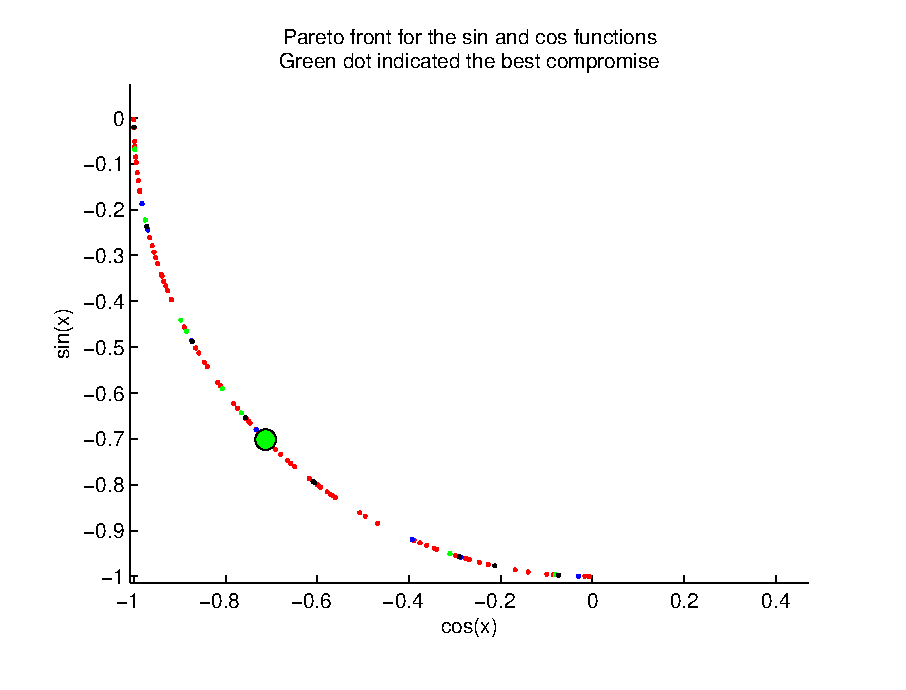
\includegraphics[width=0.85\textwidth]{SinCosPareto}
         \caption{All good compromises for the minimum of the \emph{two}
         objective functions $\sin(x)$ and $\cos(x)$, in function value
         space. Note that the green dot is closest to the origin,
         and thus indicates the ``most efficient'' compromise.}
         \label{fig:SinCosPareto}
\end{figure}

\begin{figure}[ht]
         \centering
         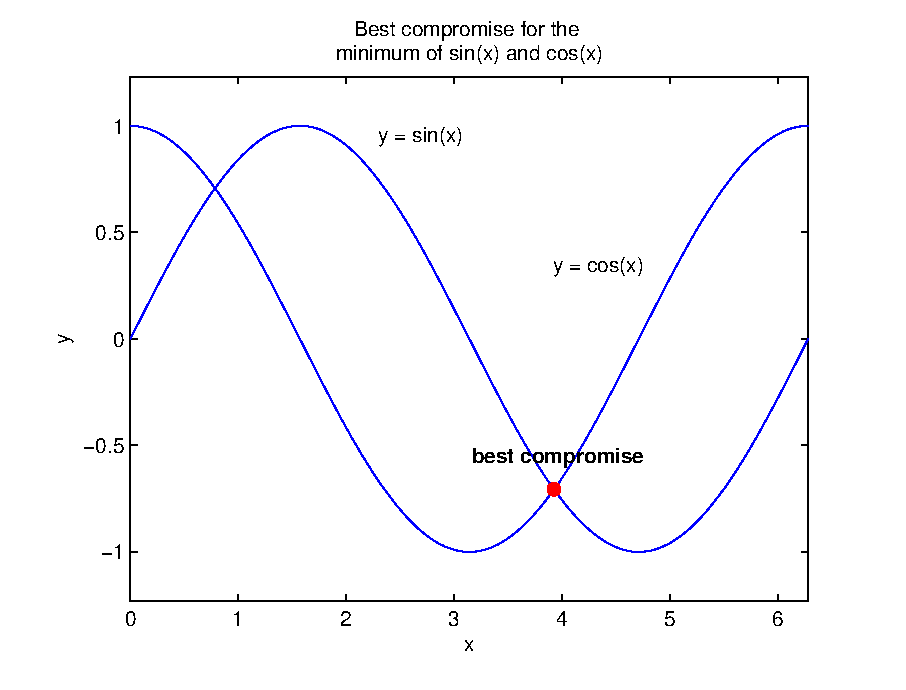
\includegraphics[width=0.85\textwidth]{SinCos}
         \caption{Best compromise for the minimum of the \emph{two}
         objective functions $\sin(x)$ and $\cos(x)$, in decision
         variable space.}
         \label{fig:SinCos}
\end{figure}
�\\
There are several algorithms that find the complete Pareto front
in multi-objective optimization problems. The most popular,
easiest to implement and most efficient one known, still is the
Non-dominated Sorting Genetic Algorithm~II (NSGA-II). This
algorithm sorts the current population according to the amount of
solutions that \emph{dominate} each other individual, Dominance of
one individual $x_i$ over another $y_i$, denoted as $x_i \prec
y_i$, is defined as

\begin{eqnarray*}
  x_i \prec y_i &\textrm{ if}& f_j(x_i) \leq f_j(y_i) \quad
  \textrm{for all functions } j, \\
 &\textrm{ and}& f_j(x_i) < f_j(y_i) \quad \textrm{for at least
 \emph{one} function } j.
\end{eqnarray*}

The NSGA-II algorithm iterates the following steps until all
solutions are non-dominated:

\begin{enumerate}

\item Create an offspring population $Q$ from the parent
population $P$ with the usual crossover and mutation operators
from a GA.

\item Count the number of solutions $y_i$ that dominate the
current solution $x_i$. Do this for \emph{all} individuals from
\emph{both} the parent population $P$ and the offspring population
$Q$.

\item Some solutions will be found to have \emph{zero} other
solutions dominate them. They are \emph{non-dominated}, and thus
part of the Pareto front of the current populations. The solutions
that have only one other solution dominate them, would have been
part of the Pareto front \emph{if} the members forming the true
Pareto front would not have been present. Those that have two
solutions dominate them would have formed the Pareto front if
\emph{those} solutions would also not be present, etc. Thus, the
level of domination is indicative of the quality of that solution.

\item Next, the \emph{crowding distances} are computed. These are
the \emph{average} distances between one solution and its
surrounding solutions in the function-value space.

\item Create a new population $R$, which contains individuals from
the previous two populations $P$ and $Q$, sorted by their level of
dominance. That is, first insert all Pareto members in $R$, then
those that have only one dominating solution, etc. Keep inserting
individuals until $R$ is the same size as $P$ and $Q$.

\item Create a subset $P_{i+1}$ from $R$ by a binary
\emph{tournament selection}. This selection takes two random
individuals from $R$, $a_R$ and $b_R$, and lets them
\emph{compete} using their domination level and crowding distances
as competitive factors. The ``winning'' individual is the one that
satisfies $a_R \prec_d b_R$, defined as

\begin{eqnarray*}
        a_R \prec_d b_R &\textrm{if}& rank(a) < rank(b)\\
        &\textrm{or}& (\,rank(a) = rank(b)\\
         &\textrm{ and }& \textrm{crowding\_distance}(a) >
         \textrm{crowding\_distance}(b))
\end{eqnarray*}

where $rank(\ell)$ indicates the rank, or domination level, of the
individual $\ell$. This process is repeated until the subset $S$
is full. Usually, the size of $P_{i+1}$ is taken to be half that
$Q$ and $R$.

\item Create a new offspring population $Q_{i+1}$, equal in size
as the original $P$, $Q$ and $R$, using crossover and mutation
from a GA, using members from the subset $P_{i+1}$ as parents.

\end{enumerate}

After the initialization step~1, steps~2 through~7 are repeated
until \emph{all} individuals are non-dominated. The crowding
distances in steps~4 and~6 are used to keep the \emph{spread} in
the solutions along the true Pareto front more or less
homogeneous~--~when these steps are not included, the solutions
tend to cluster together to the easiest-to-find compromise between
the objective functions.
\\�\\
The greatest advantage of NSGA-II is that the \emph{entire}
population will simply converge to the \emph{true} Pareto front,
so that the number of desired solutions can easily be controlled
by choosing a different population size. A slight drawback it has
compared to other algorithms of this sort is the computational
complexity of the computation of the number of non-dominated
solutions; it is of $O(M(2N)^2)$, where $M$ is the number of
objectives and $N$ is the population size. With careful
bookkeeping, this can be reduced to $O(MN^2)$, but still it tends
to be a problem for very large population sizes. However, with
today's standards in computation power this really poses only
minor problems.
\\�\\
Note that the genetic operators used to create $Q$ or $Q_{i+1}$
are completely separate from the other parts of the algorithm, so
$Q$ and $Q_{i+1}$ can essentially be generated with \emph{any} of
the aforementioned meta-heuristic optimizers. This fact will be
used later on.

\chapter{Problems with Meta-heuristic Algorithms}
Despite their popularity and general applicability, there are many
problems associated with meta-heuristic optimizers. One very
serious problem is \emph{premature convergence}~--~the population
converges to a point that is only a \emph{local} minimizer of the
function. Also, the NSGA-II algorithm used for multi-objective
problems might return fully non-dominated solutions, but
completely miss the problem's Pareto front; non-dominance is not a
guarantee for convergence to the Pareto front. This is
particularly true for small population sizes. For small
populations, the probability that no solution is dominated by
another, while still not being even close to the Pareto front, is
quite large. This necessitates using large population sizes, thus
requiring many function evaluations.
\\�\\
The GA, DE, PSO and ASA algorithm have various operators that try
to prevent this problem. In GA, it is the mutation operator that
sometimes generates a solution very far from the other population
members, increasing its robustness. In PSO, it is the fact that
sometimes solutions get assigned very large changes in their
velocities, especially when being very far removed from the
attractors. However, as found in the literature, premature
convergence still frequently occurs and necessitates several
re-runs to make sure the global optimum is found.
\\�\\
A fact that can also not be ignored is that people tend to ``get
used'' to the simplicity of such algorithms. It often becomes
their algorithm of choice for \emph{all} optimization problems
they encounter. Quite often, obvious caveats, simplifications and
weaknesses in the problem that can be exploited by \emph{much}
more powerful and accurate algorithms, are then ``overlooked'' or
sometimes even ignored.
\\�\\
It should be stressed that meta-heuristic algorithms do \emph{not}
aim to find the global minimum very accurately, nor do they aim to
be \emph{efficient} in terms of function evaluations; they only
aim to find a good \emph{approximation} to the problem's global
minimum or Pareto front, with high probability. For many problems,
function evaluations are \emph{very} expensive; personally I
frequently encounter functions that take several \emph{minutes} to
evaluate per trial, even on a 32-node quadcore cluster (128
processing units). In such cases it is much more fruitful (and
efficient) to analyze that problem to bits, and make some
reasonable assumptions that simplify the problem significantly,
rather than go at it ``blindly'' and just use a GA to solve it.
\\�\\
Despite these problems, they are still very useful, if only to get
a good initial approximation to the minimum, or a first idea about
the general shape of the Pareto front. They can also indicate
other promising regions in the search space, or function as a
simple test algorithm to find potential problems with the
objective functions.

\chapter{GODLIKE Algorithm}
The GODLIKE algorithm was written as an attempt to improve the
robustness of the meta-heuristic algorithms, and to do away with
the need to fine-tune the algorithm of your choice for each
optimization problem. It was also written to serve as a general
``umbrella'' function; to be able to tackle both single and multi
objective problems with a single function and in a uniform
fashion, and easily include more and different population based
methods.
\\�\\
GODLIKE stands for \textbf{G}lobal \textbf{O}ptimum
\textbf{D}etermination by \textbf{L}inking and
\textbf{I}nterchanging \textbf{K}indred \textbf{E}valuators, and
this is exactly what it does. It uses all four aforementioned
algorithms simultaneously (Linking), and after convergence of
either of them, or exceeding certain predefined limits, it takes
random members from each population and inserts then into random
other populations (Interchanging) before continuing the
optimization.
\\�\\
By using multiple optimizers simultaneously, it is essentially
equal to performing four (or more) consecutive optimizations all
at once, which already improves the chances of finding the global
optimum; The weaknesses associated with each algorithm are negated
by the strengths of another, while the strengths of all algorithms
simply add up.
\\�\\
The $interchange$-operator indeed destroys part of the convergence
properties of either of the algorithms it uses, but that is
exactly the intention~--~the convergence one of the algorithms is
experiencing might be to a local optimum, while the others might
be converging to the global solution, or other local minima. By
interchanging individuals between populations, GODLIKE introduces
\emph{immigrants} into the populations that can provide
alternative good solutions to the ones already being explored by
one of the algorithms. These immigrants can steer the population
into other, unexplored areas of the search space, increasing the
chances of locating the global minimum. By keeping the populations
separate, also the principle of \emph{isolation} is exploited
automatically~--~portions of the search space will be thoroughly
explored by one of the populations, while not affecting the other
populations.
\\�\\
The interchange operator is extremely useful for multi-objective
problems; when one population is completely non-dominated,
interchanging individuals between populations will usually result
in a \emph{dominated} population, which continues the search for
the Pareto front, in stead of reporting convergence.
\\�\\
In conclusion, GODLIKE does not aim to make either of the
algorithms more efficient in terms of function evaluations,
(rather, it tends to require \emph{more} function evaluations).
However, the \emph{robustness} was aimed for, and until now, my
simple experiments have indeed shown that hard-to-find global
optima that could almost never be found by either GA, DE, ASA or
PSO individually, \emph{could} be found by but their
\emph{combined} efforts in GODLIKE.

\section{GODLIKE in Detail}
GODLIKE was written primarily with all of the above in mind, but
also partly for me personally to \emph{finally} learn
objective-oriented programming in MATLAB. As such, the files
\texttt{pop\_single.m} and \texttt{pop\_multi.m} are indeed
\texttt{classdef}-class definitions. A slight drawback of this is
that only users who own MATLAB 2008b (or later) can use it, but I
think it is not hard (only time-consuming) to re-write these files
to pure functions.
\\�\\
GODLIKE requires four files: \texttt{GODLIKE.m},
\texttt{pop\_multi.m}, \texttt{pop\_single.m} and
\texttt{set\_options.m}.

\subsection{GODLIKE.m}
This is of course the main function. All required operations are
carried out here. The operation of GODLIKE.M is kept simple,
readable and understandable by generously using nested-functions.
All basic operations are performed in the first three cells:

\begin{description}

\item [\%\%Initialize] Here, the user-input is checked thoroughly.
Also, the user-provided objective function(s) are tested and used
to determine whether single or multi-objective is desired. Also,
the user-input is reshaped and reformatted into a form that is
assumed in all classes and functions. During this last process,
also default options and values are assigned should they be empty
or omitted.

\item [\%\%GODLIKE loop] The main loop that executes the
optimization. In this loop, the amount of individuals per
optimizer, and the number of iterations that is to be carried out
by each optimizer, is selected by randomly ``breaking up'' the
user-selected (or default) values. For example, if 100 individuals
are to be used in the algorithms GA, DE, and PSO, the algorithms
get assigned for instance [45, 13, 42] or [6, 22, 72] individuals.
Note that these numbers are chosen differently at every iteration.
\\�\\
Next, using these values, the number of desired populations are
created (objects of type \texttt{pop\_single.m} or
\texttt{pop\_multi.m} are instantiated). Then, GODLIKE performs
the randomly selected number of iterations in each algorithm,
keeping track of the convergence of either of them. For single
objective optimization, convergence is said to have been achieved
if the decrease in the global minimum found so far is less than
[\texttt{options.MinDescent(1)}] for at least
[\texttt{options.MinDescent(2)}~*~\texttt{options.MinDescentMultiplier}]
iterations (see \texttt{set\_options} below). For multi-objective
optimization, convergence of an algorithm occurs simply when all
members of that population are non-dominated.
\\�\\
After all algorithms have been run for the said amount of
iterations, convergence of the GODLIKE loop is checked in a
similar manner: for single-objective optimization, if the amount
if GODLIKE iterations is larger than [\texttt{options.MinIters}]
and the decrease in the global optimum is less than
[\texttt{options.MinDescent(1)}] for at least
[\texttt{options.MinDescent(2)}] GODLIKE iterations, the GODLIKE
loop is terminated. For multi-objective problems, at least
[options.MinIters] GODLIKE iterations will be performed, and if
after said amount of iterations all solutions are non-dominated,
the GODLIKE loop is terminated. Note that the GODLIKE loop is also
terminated when more than [\texttt{options.MaxIters}] iterations
have been performed, or when more than
[\texttt{options.MaxFunEvals}] function evaluations have been
executed at any point in the loop.
\\�\\
Every next GODLIKE iteration again randomly selects the number of
individuals and iterations per algorithm to be carried out. Only
this time, the existing populations are first \emph{shuffled};
that is, the $interchange$-operator is applied.

\item [\%\%output values] Simply assigns the desired output
variables. These are updated every iteration, but only properly
formatted and nicely cut into pieces by the operations in this
cell, before they are returned to the user.

\end{description}

Note that the operation manual (how to actually use GODLIKE in
MATLAB) is included in a separate PDF-file (\texttt{manual.pdf}).
The nested functions are where the actual work is carried out.
Note also the nested function \texttt{display\_progress}: this is
called only when [\texttt{options.display}] is set to 'plot' or
'on'.

\subsection{pop\_single.m} A SubClass of the \texttt{handle}
class, this is the file where all the actual optimizations are
carried out. It constructs a ``population'' called \texttt{pop},
which has properties

\begin{description}

  \item[algorithm] the optimization algorithm used (either 'GA',
  'PSO', 'DE' or 'ASA').

  \item[funfcn] The objective function.

  \item[individuals] All members of the population.

  \item[fitnesses] their corresponding objective function values

  \item[size] population size (number of individuals).

  \item[lb] lower bounds,

  \item[ub] upper bounds. Note that both the lower and upper
  bounds are replicated and resized upon initiazation, to conform
  to the size [popsize $\times$ dimensions]. This does away with
  the need to constantly replicate them for operations like
  \texttt{check\_bounds}, or re-initializing individuals as is done
  in some of the algorithms.

  \item[dimensions] The dimensions of the problem.

  \item[funevals] Total number of function evaluations made

  \item[iterations] Total number of iterations so far performed

  \item[options] A copy of the options structure (see \texttt{set\_options})

  \item[pop\_info] A structure to store intermediate data and pass
  it from method to method. For single-objective optimization, it
  contains the following fields:
  \begin{itemize}
    \item parent\_population
    \item offspring\_population
    \item function\_values\_parent
    \item  function\_values\_offspring
  \end{itemize}

  Note that the fields \texttt{parent\_population} and
  \texttt{function\_values\_parent} are only here for completeness and
  consistent programming, their contents is completely the same as the class
  properties \texttt{individuals} and \texttt{fitnesses}.

\end{description}

These properties are all assigned by the constructor (when
properly called). The constructor also creates the initial
population of randomly generated individuals within the given
bounds, and evaluates the function for these initial individuals.
Note that the constructor does not perform any elaborate checks on
the given input; it relies on the fact that this has already been
done in \texttt{GODLIKE.m}.
\\�\\
On a population \texttt{pop}, the following methods can be
applied:

\begin{description}

  \item[iterate (Public)] Perform one single-objective iteration.
  Aside from the constructor, this is actually the only method directly
  accessed in \texttt{GODLIKE.m}; all other methods are only used
  \emph{within} \texttt{pop\_single.m}.

  \item[create\_offspring (Hidden)] Creates offspring from the
  parent population, using the pre-set algorithm. These offspring are
  inserted into the \texttt{pop\_info} structure. Note that this
  contains only the \emph{first half} of all the optimization
  algorithms.

  \item[evaluate\_function (Hidden)] Proper evaluation of the
  objective function. Function can be evaluated in two
  distinct ways, each of these requiring implementation in \texttt{pop\_single}.
  The correct one has been determined in GODLIKE, which is passed to
  \texttt{pop\_single} in the background via the \texttt{options} structure.

  \item[replace\_parents (Hidden)] Selective replacement of the
  parent population; the exact replacement procedure depends on the selected
  algorithm. Note that the \emph{second half} of the algorithms is
  carried out here.

  \item[check\_bounds (Hidden)] Checks whether offspring is generated within the given
  bounds \texttt{lb} and \texttt{ub}. Also, for PSO specifically,
  the bounds on the new velocities are checked.

  \item[initialize\_algorithms (Hidden)] PSO and ASA need some
  additional initialization (temperature, velocities, ...). With future expansions
  of GODLIKE in mind, I thought I make a separate method for this.

\end{description}


\subsection{pop\_multi.m} A SubClass of
\texttt{pop\_single.m}. Inherits all the methods defined therein,
and is constructed in exactly the same way. It adds only one
property \texttt{num\_objectives}, and the two methods
\texttt{non\_dominated\_sort} and \texttt{tournament\_selection}.
\\�\\
Note that the methods \texttt{evaluate\_function},
\texttt{initialize\_algorithms} and \texttt{iterate} are
overloaded in \texttt{pop\_multi.m}. This is required because
multi-objective functions need to be evaluated differently (there
may be multiple functions, or a single function with
two-dimensional output), one iteration now must call
\texttt{non\_dominated\_sort} and \texttt{tournament\_selection}
in stead of \texttt{replace\_parents}, and the PSO-algorithm must
be initialized and used differently (see below).

\section{PSO in Multi-objective Optimization}
Using the ASA and DE optimizers (in stead of the usual GA) to
create offspring populations for the NSGA-II method is quite
straightforward. However, the PSO algorithm is more demanding; it
needs to have some values for $lbest$, $gbest$ and $nbest$, which
are not defined in an obvious way for multi-objective
optimization. There are several papers in the literature that deal
with this very problem. Some find reasonable results, but most
perform quite poorly compared to similar algorithms. The best one
I could find relied on a completely different algorithm (so
\emph{not} NSGA-II), so for the time being, I chose to use
another, worse one, that \emph{did} fit in GODLIKE's NSGA-II
context.
\\�\\
But, it is particularly in this context that PSO seems rather
unsuited for the task. To remedy the problem with $lbest$, $gbest$
and $nbest$, the following criteria seemed to work best:

\begin{itemize}

\item only update $lbest$ if the new individual dominates the
previous $lbest$, \emph{and} if it is part of the current
population's Pareto front ($rank = 0$)

\item only update $gbest$ with one of the members of the current
Pareto front, that has a larger crowding distance than the
previous $gbest$.

\item For every iteration, find the
\texttt{options.num\_neighbors} individuals that are closest in
function-value space to the current individual. These form the
individual's \emph{new neighbors}. The best of these neighbors,
$nbest$, dominates all other neighbors and has the largest
crowding distance.

\end{itemize}

Despite these remedies, PSO remains the least powerful algorithm
for multi-objective optimization; it doesn't really seem to be
able to achieve convergence.

\section{Known Problems and Issues} As mentioned above, using the PSO
algorithm on multi-objective problems should be done sparingly, or
at least in conjunction with another algorithm. Initially it seems
to push the solutions towards the Pareto front quite fast, but I
think this is more due to the non-dominated sorting and tournament
selection. It is very hard to get convergence with PSO, but in
conjunction with DE it does work reasonable.
\\�\\
The 'A' in (A)SA is really not deserved. Basically I just used the
simulated annealing written by Joachim Vandekerckhove (also on the
FEX, file ID\#10548) and rewrote it to be suited for populations.
Adapting the control parameters at each iteration, which is the
true power of ASA, is not included now. As such it is probably the
weakest algorithm for single-objective optimization, and the
second-worst in multi-objective problems. However, I found it to
still be useful sometimes, as it generates many solutions in
\emph{all} regions of low function value.
\\�\\
For very large population sizes, the crossover operator in GA
seems to take up very much computation time. I have no idea why
that is, so if you do know why, please let me know. Also, the
to-and-fro conversion between binary and real representations is
relatively costly. While this is probably not a problem (the
effect only becomes noticeable for population sizes larger than
$\sim$4000), it's still something I'm baffled about. If anyone
knows a better way to do it, please let me know.

\section{Future Work} Currently, GODLIKE only accepts objective
functions, be it one or many. In the near future, I think it is
most important to include the possibility to also pass it
constraint functions. In the current form, penalty-function
methods must be used to incorporate constraint functions, but this
is certainly not the best way to do it.
\\�\\
Naturally, I need to do some more research on using PSO in
multi-objective problems. It was found to be quite promising in
the literature despite the implementation difficulties, but the
current implementation in GODLIKE does not really solve the
problems satisfactorily.

\end{document}
